\documentclass[12pt,a4paper]{scrartcl}
\usepackage[utf8]{inputenc}
\usepackage[T1]{fontenc}
\usepackage{lmodern}
\usepackage[ngerman]{babel}
\usepackage{graphicx}
\addtokomafont{disposition}{\rmfamily}

\title{Richtungsanzeiger}
\subtitle{Technischer Entwurf}
\author{Jonas Tochtermann}
\date{\today}
\begin{document}

\maketitle

\section{Funktionale und nicht-funktionale Anforderungen}

% Beschreiben Sie die funktionalen und nicht-funktionalen Anforderungen wie folgt:
% A. Bilden Sie die funktionalen Anforderungen als vollständiges Anwendungsfalldiagramm (Use Case) nach UML ab.
% B. Beschreiben Sie jeden Akteur mit einem Satz.
% C. Beschreiben Sie die nicht-funktionalen Anforderungen (Qualitätsanforderungen) nach FURPS. Jede Anforderung muss messbar sein. Es sind mindestens drei nicht-funktionale Anforderungen zu erfassen.

\subsection{Funktionale Anforderungen}

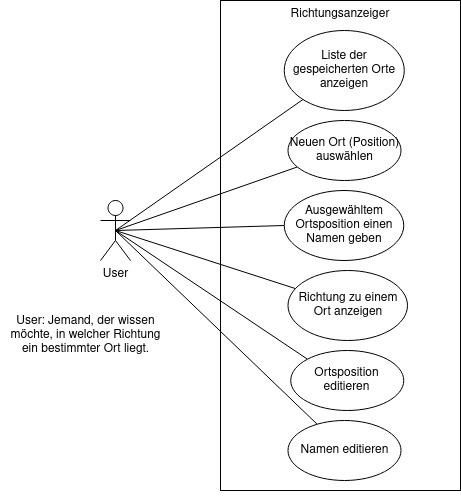
\includegraphics[width=10.0cm]{../UseCase.jpg}

\subsection{Nicht-funktionale Anforderungen}

\begin{itemize}
  \item Die Sprache der Benutzeroberfläche ist Deutsch.
  \item Persistente Daten werden mit SharedPreferences verwaltet.
  \item Zielplattform ist Android 8.1.
  \item Die App wird in Java implementiert.
\end{itemize}

\section{Testkonzept}

% Stellen Sie ein Testkonzept auf, welches beschreibt, wie Sie Ihre Applikation auf deren Funktionalität und Qualität überprüfen wollen. Folgende Bedingungen werden an das Testkonzept gestellt:
% A. Beschreiben Sie das Testumfeld genau.
% B. Beschreiben Sie die Testmethode.
% C. Beschreiben Sie mindestens für jeden Anwendungsfall einen aussagekräftigen Testfall mit
%   a. Identifikation
%   b. Vorbedingungen
%   c. Schritt-für-Schritt-Vorgehen (Aufzählung)
%   d. Erwartetes Resultat

\begin{description}
  \item [Womit wird die App getestet?] Wahrscheinlich allein mit dem Emulator (Nexus 6 mit Android 8.1, API-Level 27); falls sich noch die Möglichkeit ergibt, ein Android-Phone aufzutreiben, würde gegebenenfalls auch dieses zum Einsatz kommen.
  \item [Wie wird die App getestet?] Manuelle und automatisierte Tests. Bei den hier aufgeführten manuellen Tests wäre es sinnvoll, auch die Möglichkeit der Automatisierung zu berücksichtigen.
\end{description}

\subsection{Testfälle}

\begin{enumerate}
  \item Liste der gespeicherten Orte anzeigen

  \begin{description}
    \item [Identifikation] showList
    \item [Vorbedingungen] Bei der Installation werden zwei Orte (Matterhorn und Bundeshaus) mitgegeben, sodass die Liste bereits beim ersten Öffnen einen Inhalt besitzt.
    \item [Vorgehen] Automatisierter Test zur Überprüfung, ob beim Anzeigen der MainActivity eine Liste mit Inhalt angezeigt wird.
    \item [Erwartetes Resultat] Die Liste mit den \dq installierten\dq  Orten (inklusive aller Icons: Kompass und Stift) wird angezeigt.
  \end{description}

  \item Neuen Ort (Position) auswählen

  \begin{description}
    \item [Identifikation] pickPosition
    \item [Vorbedingungen] Eine KartenApp ist auf dem Test-Phone vorhanden und brauchbar für eine Datenein- und -ausgabe zwischen Activities. Die MainActivity mit der Liste wird angezeigt. Der Testfall showList ist erfolgreich durchgeführt worden.
    \item [Vorgehen] Manueller Test; Drücken auf den \dq Ort hinzufügen\dq -Button, Eingabe \dq ZLI\dq im Suchfeld, Drücken auf \dq Position übernehmen\dq -Icon.
    \item [Erwartetes Resultat] Die EditLocationActivity wird angezeigt mit den Koordinaten \dq 47.3598043 N\dq  (Breitengrad) und \dq 8.5210211 O\dq  (Längengrad). Die Angaben dürfen eine Abweichung von +/- 0.001 aufweisen.
  \end{description}

  \pagebreak

  \item Ausgewählter Ortsposition einen Namen geben

  \begin{description}
    \item [Identifikation] pickName
    \item [Vorbedingungen] Der Testfall pickPosition wurde ausgeführt und die EditLocationActivity wird angezeigt.
    \item [Vorgehen] Manueller Test; Im Feld mit dem Platzhalter \dq Name des Ortes\dq  wird \dq ZLI\dq  eingegeben, danach wird auf das Icon \dq Speichern und zurück zur MainActivity\dq  geklickt.
    \item [Erwartetes Resultat] Die aktualisierte Liste mit dem neuen Eintrag \dq ZLI\dq  wird angezeigt.
  \end{description}

  \item Richtung zu einem Ort anzeigen

  \begin{description}
    \item [Identifikation] showDirection
    \item [Vorbedingungen] Der Testfall showList wurde durchgeführt. In den Einstellungen des Emulators wird als Location Basel (47.5596N, 7.5886O) genommen. Die MainActivity wird angezeigt.
    \item [Vorgehen] Manueller Test; Auf der Liste wird mit Klick auf das entsprechende Kompass-Icon \dq Matterhorn\dq  ausgewählt.
    \item [Erwartetes Resultat] Die ShowDirectionActivity wird angezeigt mit dem Kompass und der Richtungsanzeige auf 178°. Auf dem Emulator sollte Norden gegen \dq Oben\dq  sein.
  \end{description}

  \item Ortsposition bearbeiten

  \begin{description}
    \item [Identifikation] editPosition
    \item [Vorbedingungen] Der Testfall showList wurde durchgeführt. Die MainActivity wird angezeigt.
    \item [Vorgehen] Manueller Test; Auf der Liste wird mit Klick auf das entsprechende Stift-Icon \dq Bundeshaus\dq  ausgewählt. Nun sollte die EditLocationActivity angezeigt werden. Mit Klick auf \dq Ort auswählen\dq  wird auf die SearchOnMapActivity gewechselt. Im Suchfeld \dq Freibad Marzili\dq  eingeben. Drücken auf \dq Position übernehmen\dq -Icon.
    \item [Erwartetes Resultat] Die EditLocationActivity wird angezeigt mit den Koordinaten \dq 46.9424203 N\dq  (Breitengrad) und \dq 7.4437811 O\dq  (Längengrad). Die Angaben dürfen eine Abweichung von +/- 0.001 aufweisen.
  \end{description}

  \item Ortsnamen bearbeiten

  \begin{description}
  \item [Identifikation] editName
  \item [Vorbedingungen] Der Testfall editPosition wurde durchgeführt. Die EditLocationActivity wird angezeigt.
  \item [Vorgehen] Manueller Test; Die TextView mit dem Namen wird ausgewählt. Anstelle des bisherigen Textes wird \dq Marzilibad\dq  eingegeben, danach wird auf das Icon \dq Speichern und zurück zur MainActivity\dq  geklickt.
  \item [Erwartetes Resultat] Die aktualisierte Liste mit dem geänderten Eintrag \dq Marzili\dq  wird angezeigt.
  \end{description}

\end{enumerate}

\section{Aufbau des Systems}

% Beschreiben Sie den Aufbau des Systems in einem Klassen- oder Paketdiagramm.
% A. Das Klassen- oder Paketdiagramm ist verständlich und mehrheitlich nach UML.
% B. Das Diagramm bildet die Beziehungen ab.
% C. Das Diagramm und die Implementation passen zusammen.

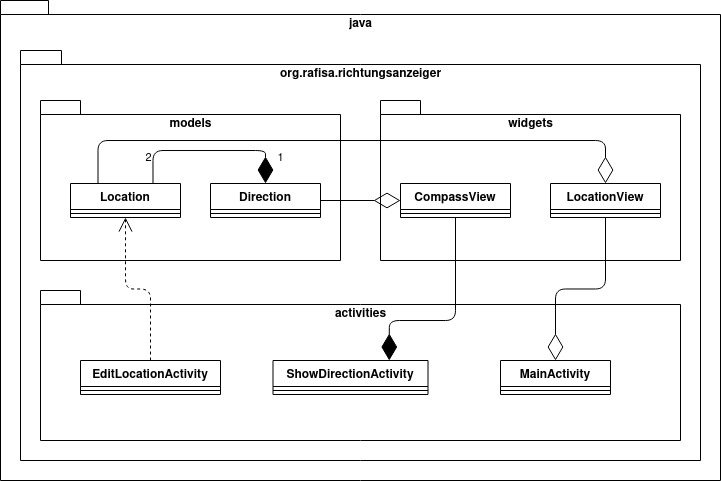
\includegraphics[width=15.0cm]{../system.jpg}

% \section{Visualisierung des Gesamtsystems}
%
% Das Gesamtsystem wurde als Verteilungsdiagramm (Deployment-Diagramm) oder sonst einer verständlichen Grafik visualisiert. Aus der Abbildung lassen sich mindestens folgende Informationen herauslesen:
% A. Einzelteile des Systems.
% B. Beschreibung der eingesetzten Technologien und Komponenten.
% C. Beschreibung der Schnittstellen und Abhängigkeiten der einzelnen Teile.
% D. Beschreibung der Protokolle.
%

\end{document}
